
\(h(x) = -x^3 + 30x^2 - 108x - 490\).

\subsection*{1.}

\(h(x)\) est un polynôme dérivable sur \(\mathbb{R}\), donc sur \([-6 \,;\, 26]\), et sur cet intervalle :
\[
h'(x) = -3x^2 + 2 \times 30x - 108 = -3x^2 + 60x - 108.
\]

\subsection*{2.}

\paragraph{a.} \(\mathcal{C}'\) est la représentation graphique d'une fonction trinôme : c'est donc une parabole tournée vers le bas : c'est donc \(\mathcal{C}_1\).

Comme \(h'(x) \geqslant 0\) sur \([2 \,;\, 18]\), \(h\) est croissante sur cet intervalle et sa représentation n'est pas \(\mathcal{C}_3\) ; c'est donc \(\mathcal{C}_2\).

\paragraph{b.} On a :
\begin{align*}
h'(x) &= -3 \left( x^2 - 20x + 36 \right) \\
&= -3 \left[ (x - 10)^2 - 100 + 36 \right] \\
&= -3 \left[ (x - 10)^2 - 64 \right] \\
&= -3 \left[ (x - 10)^2 - 8^2 \right] \\
&= -3 (x - 10 + 8)(x - 10 - 8) \\
&= -3 (x - 2)(x - 18).
\end{align*}
\(h'(x) = 0\) pour \(x = 2\) et \(x = 18\), mais \(h(10) = -3 \times 8 \times (-8) = 252\) : c'est donc \(\mathcal{C}_1\).

\begin{center}
\psset{xunit=0.3cm,yunit=0.003cm,labelFontSize=\scriptstyle,labelsep=0.1pt}
\begin{pspicture}(-11,-800)(35,1625)
\psaxes[linewidth=0.95pt,Dx=2,Dy=200]{->}(0,0)(-10,-800)(31.5,1625)
\def\Func{ x x x neg 30 add mul  108 sub  mul 490 sub }
\psplot[plotpoints=1000,linewidth=1.25pt,linecolor=blue]{-6}{26}{\Func}
\psplot[plotpoints=1000,linewidth=1.25pt,linecolor=blue,linestyle=dashed]{-6}{26}{x x 3 neg mul 60 add mul 108 sub}
\psplot[plotpoints=1000,linewidth=2pt,linecolor=blue, linestyle=dotted]{-6}{26}{x x 3  mul 60 sub mul 108 add}
\psplot[plotpoints=1000,linewidth=1.25pt,linecolor=red]{-6}{2.87}{-108 x mul -490 add}
\uput[ul](26.5,640){$\mathcal{C}_3$} \uput[u](12.,940){$\mathcal{C}_2$} \uput[ur](-6,-450){$\mathcal{C}_1$} \uput[ur](2.87,-750){$\mathcal{T}$}
\end{pspicture}
\end{center}

\subsection*{3.}

\begin{align*}
&M(x \,;\, y) \in \mathcal{T} \\
\iff &y - h(0) = h'(0)(x - 0) \\
\iff &y - (-490) = -108x \\
\iff &y = -108x - 490.
\end{align*}

\subsection*{4.}

On a vu que \(h'(x) = -3(x - 2)(x - 18)\) : ce trinôme est négatif sauf entre les racines 2 et 18.

La fonction \(h\) est donc décroissante sauf sur l'intervalle \([2 \,;\, 18]\), où elle est croissante.

\begin{center}
\begin{tikzpicture}
\tkzTabInit[lgt=3.5, espcl=3.5]{$x$ / 1, {Signe de $h'(x)$} / 1, {$h(x)$} / 2}{${-6}$, ${2}$, ${18}$, ${26}$}
\tkzTabLine{,-,0,+,0,-,}
\tkzTabVar{+/{$1454$},-/{$-594$},+/{$1454$},-/{$-594$}}{/}
\end{tikzpicture}
\end{center}

